\documentclass[10pt]{article}
\usepackage{tikz}
\usepackage{xcolor}
\usepackage{hyperref}
\hypersetup{
    colorlinks=true,
    linkcolor=blue
}


% \usepackage[paperwidth=2in, paperheight=4in, margin=1in]{geometry}
\usepackage{pdfpages}
\usepackage[style=ieee, isbn=false, citestyle=numeric-comp, backend=biber]{biblatex}

%%% TODO: Change the following line to reference your BibTex library file.
\addbibresource{my-collection.bib}

\AtEveryBibitem{
 \clearname{issn}
 \ifentrytype{book}{}{
  \clearlist{publisher}
  \clearname{editor}
 }
 }
\usepackage{enumitem}
\setlist[itemize]{itemsep=0.25em, topsep=0pt}

\usepackage[letterpaper, margin=1in]{geometry}
\usepackage[utf8]{inputenc}
\usepackage{fontspec}
\usepackage{indentfirst}
\usepackage{soul}
\usepackage{booktabs}
\setmainfont{Verdana}
\usepackage{etoolbox}
\usepackage[explicit]{titlesec}

\usepackage{fancyhdr}
\makeatletter
\patchcmd{\f@nch@head}{\rlap}{\color{gray}\rlap}{}{}
\makeatother

\pagestyle{fancy}
\fancyhf{}
\renewcommand{\headrulewidth}{0pt}
\fancyhead[R]{\thepage}

\newcommand\D{\hangindent1.25cm}

\newlength\mylena
\newlength\mylenb
\setlength\mylena{1.25cm}
\setlength\mylenb{\dimexpr\textwidth-\mylena\relax}

\newcommand\PlaceNumber[1]{%
  \makebox[\mylena][l]{#1}}
  
\renewcommand{\thesection}{\Roman{section}}
\titleformat{\section}
    {\normalfont\bfseries}
    {}
    {0em}
    {\PlaceNumber{\thesection.}\parbox[t]{\mylenb}{\raggedright#1}}
    % [\vspace*{5pt}]

\titleformat{name=\section,numberless}
    {\normalfont\bfseries}
    {}
    {0em}
    {\parbox[t]{\mylenb}{\raggedright#1}}
    % [\vspace*{5pt}]
    
    % {}
    % {0em}
    % {\PlaceNumber{\thesection.}\parbox[t]{\mylenb}{\raggedright#1}}
    % [\vspace*{5pt}]
    
\renewcommand{\thesubsection}{\Alph{subsection}}
\titleformat{\subsection}
    {\normalfont}
    {}
    {0em}
    {\hspace{1.25em}\PlaceNumber{\thesubsection.}\parbox[t]{\mylenb}{\raggedright#1}}
    
\titleformat{name=\subsection, numberless}
    {\normalfont}
    {}
    {0em}
    {\parbox[t]{\mylenb}{\raggedright#1}}
    
\renewcommand{\thesubsubsection}{\arabic{subsubsection}}
\titleformat{\subsubsection}
    {\normalfont}
    {}
    {0em}
    {\hspace{2.5em}\PlaceNumber{\thesubsubsection.}\parbox[t]{\mylenb}{\raggedright#1}}
    
\renewcommand{\theparagraph}{\alph{paragraph}}
\setcounter{secnumdepth}{4}

% \renewcommand{\theparagraph}{\alpha{paragraph}}
\titleformat{\paragraph}
    {\normalfont}
    {}
    {0em}
    {\hspace{3.5em}\PlaceNumber{\theparagraph.}\parbox[t]{\mylenb}{\raggedright#1}}
    
    
\setlength{\parskip}{1em}
\setlength{\parindent}{0em}

\DeclareRobustCommand{\todo}[1]{{\sethlcolor{yellow}\hl{\textbf{TODO:} #1}}}


\begin{document}

% \maketitle
\begin{center}
    
\textbf{{\large Form}}

\textbf{{\large Application for Reappointment, Tenure, and/or Promotion}}

{\footnotesize [Approved by the Faculty Senate 4/98. Revised 3/04; 08/11; 03/15; 6/17; 5/19]}
\end{center}

Procedures for the RTP  process will be governed by pertinent sections in Chapter IV in the Faculty Handbook.  

Name of RTP candidate: Lucas Layman

Department: Computer Science

Personnel action applied for: Reappointment at the rank of Assistant Professor

\setlength{\parskip}{0cm}
Effective date:	Aug 2017--May 2021

End of current contract period: May 2021

End of current academic year: 2020--2021

\section{Academic Status at UNCW}
\setlength{\parindent}{1.25cm}
\setlength{\parskip}{0cm}

Present rank: Assistant Professor

Effective date: August 7, 2017

Previous rank(s) and date(s) at UNCW: None

\D Current employment status: Nontenured, fourth year of initial five-year appointment--reappointment application deferred one year for Family Medical Leave.

\section{Education}

\begin{table}[!h]
\centering
\begin{tabular}{@{}llll@{}}
\toprule
Institution                       & Concentration      & Dates     & Degree \\ \midrule
North   Carolina State University & Computer   Science & 2004-2009 & Ph.D.  \\
North   Carolina State University & Computer   Science & 2002-2004 & M.S.   \\
Loyola   College (now Loyola University)                  & Computer   Science & 1998-2002 & B.S.   \\ \bottomrule
\end{tabular}
\end{table}

\section{Professional History (other than UNCW)}

\begin{table}[!h]
\centering
\begin{tabular}{@{}lll@{}}
\toprule
Position/Rank               & Institution                        & Dates     \\ \midrule
Senior   Research Scientist & Fraunhofer   USA, Inc.             & 2009-2017 \\
Research   Associate        & National   Research Council Canada & 2009      \\ \bottomrule
\end{tabular}
\end{table}

\newpage
\section{Contributions to Teaching}

\setlength{\parindent}{1.25cm}
\subsection{Required subcategories:}
\subsubsection{Courses taught (a non-chronological list of course numbers and titles)}

\begin{table}[!h]
\centering
\begin{tabular}{@{}lll@{}}
\toprule
Course number & Title                             & Term(s)                  \\ \midrule
CSC 231       & Introduction   to Data Structures & SP21, FA20, SP20, SP19, SP18 \\
CSC 242       & Computer   Organization           & FA18, SP18, FA17         \\
CSC 315       & Mobile   Applications Development & SP21, FA20, SP20, SP19, FA18 \\
CSC 350 	  & Secure Programming				  & SP21					\\
CSC 475/592   & Engineering Secure Software     & SP19                     \\ \bottomrule
\end{tabular}
\end{table}


\subsubsection{Sample course materials. Identify the materials you have uploaded on the secure RTP electronic website (e.g., course syllabus, tests, modules).}
\begin{center}
	\color{blue} Text in blue are links to Supporting Materials
\end{center}

\newlength{\bulletindent}
\setlength{\bulletindent}{3.25cm}
\setlength{\parindent}{2.25cm}

\textbf{CSC 231 -- Introduction to Data Structures}
\setlength{\leftmargini}{\bulletindent}
\begin{itemize}
    \item \hyperref[CSC 231 Syllabus]{Syllabus}
    \item Module – ArrayList data structure: \hyperref[CSC 231 ArrayList Worksheet]{ArrayList worksheet}, \hyperref[CSC 231 ArrayList data structure - Stacks-Queues-Deques slides]{slides}
\end{itemize}

\vspace{1em}
\textbf{CSC 242 -- Computer Organization}
\begin{itemize}
    \item \hyperref[CSC 242 Syllabus]{Syllabus}
\end{itemize}



\subsubsection{Summary of student evaluations since last personnel action at UNCW:}
\begin{figure}[!h]
	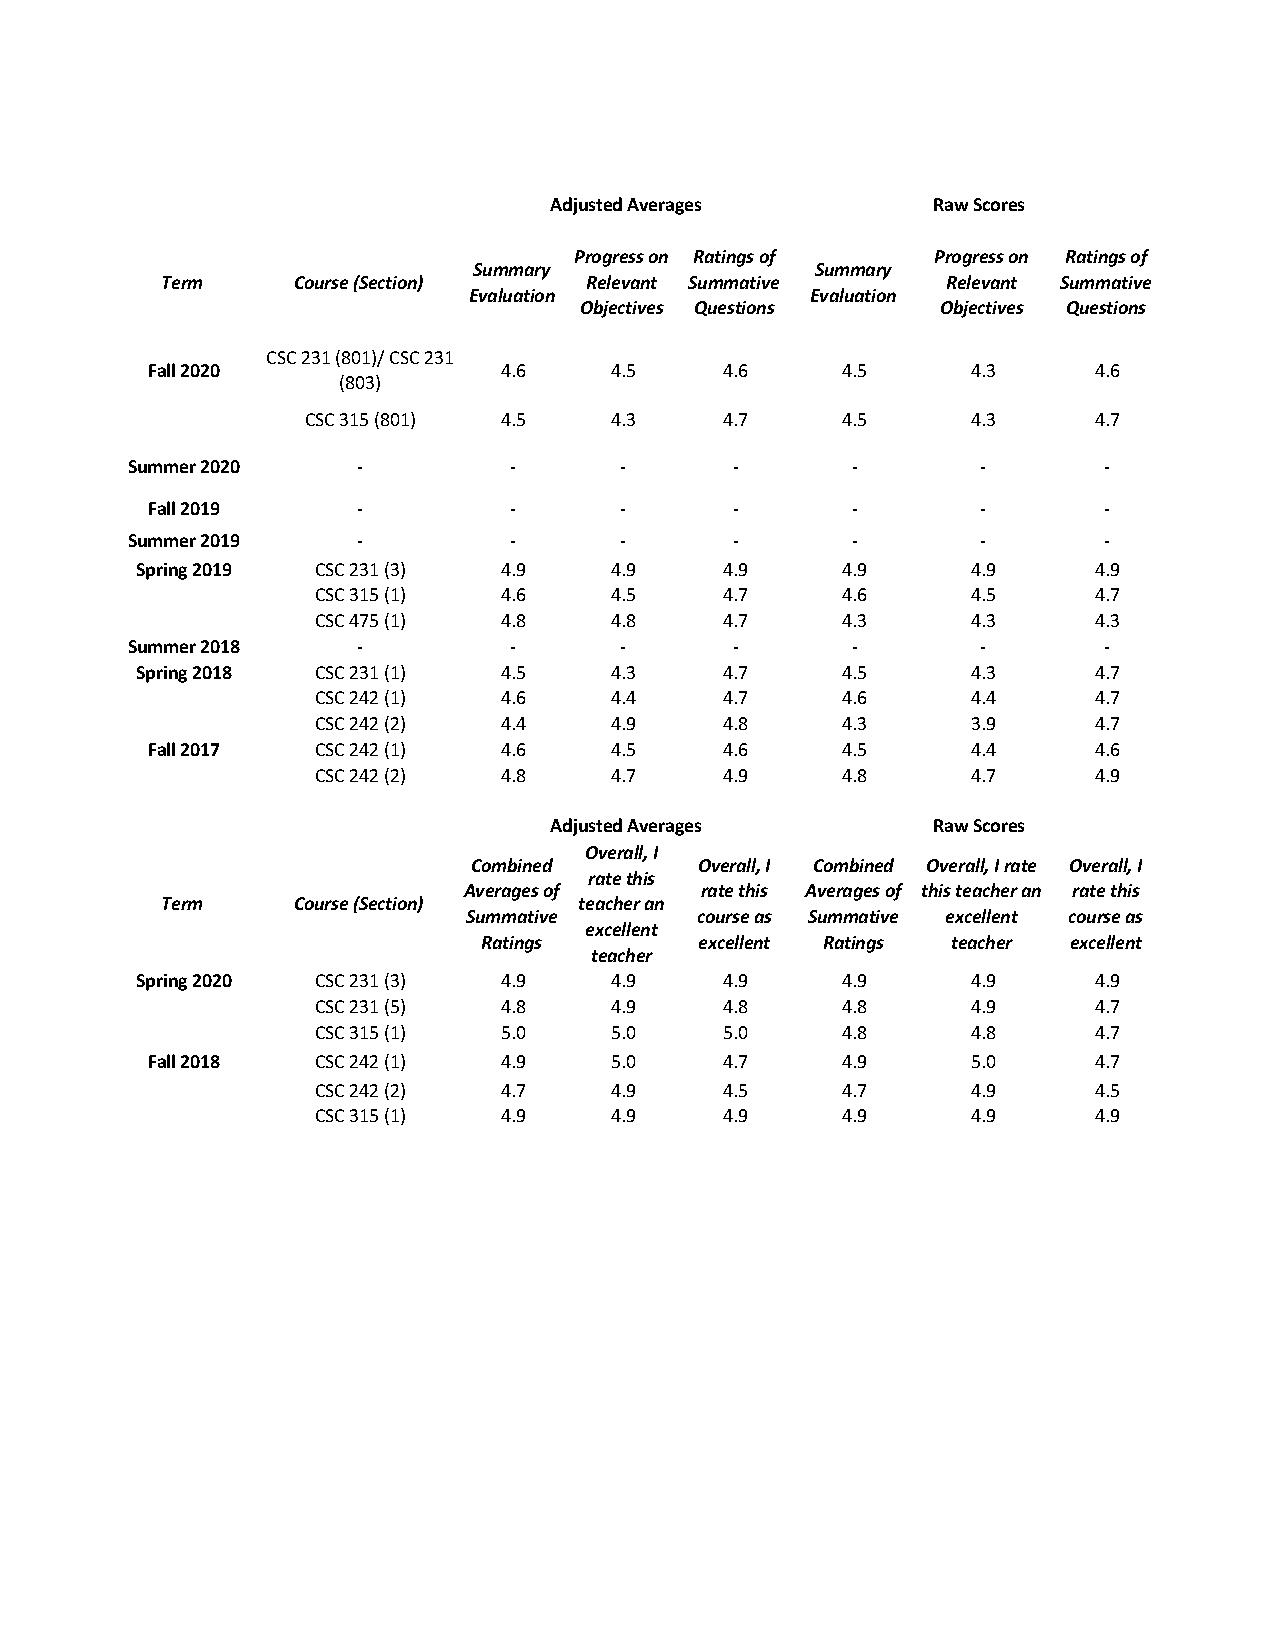
\includegraphics[scale=1.0]{IDEASummaryTable}
\end{figure}


\subsubsection{Peer evaluations of teaching  since last personnel action at UNCW. Include the name of the evaluator, rank/position, course observed, and date. (Upload a copy of all peer evaluations and any appended responses by the candidate to the designated RTP electronic website).}

\begin{itemize}
    \item Assoc. Prof. Devon Simmonds, CSC 242 – Computer Organization, 16 October 2017 - \hyperref[Fall 2017 Peer Observation]{Link to Supporting Materials}
\end{itemize}

\subsubsection{Reflective analysis of teaching strengths and actions taken to implement improvements. (Limit to a maximum of three examples and no more than one page in total.)}

\newlength{\innerparindent}
\setlength{\innerparindent}{2.1cm}
% \setlength{\parindent}{\innerparindent}

\renewcommand\D{
    \hangindent\innerparindent
    \setlength{\parskip}{1em}
    \setlength{\parindent}{\innerparindent}
    }


\D \textbf{My biggest strength is that I listen to the students}. When they are confused or disengaged with the material, that is because I have not communicated well, so I ask questions and go over the topic again. When the same quiz question is answered incorrectly many times, the problem is most likely with the question or my delivery. If students are not coming to me with questions, I have not motivated them enough. If students offer feedback that an assignment was kind of boring, then I need to revise my assignment. I care deeply about the students' success, and the best way to help them is to listen to their issues and adjust to their needs. Students are good at detecting and, usually, reciprocating the instructor's effort. I do my best to be open and inviting to the students, but many remain reluctant to ask for help. I have implemented a few practices to open other channels of feedback and communication:
\begin{enumerate}
    \item In CSC 231 -- Introduction to Data Structures, most programming assignments and quizzes are \textbf{automatically graded by testing programs} that I give to the students. The test programs help the students debug their code, and also produce scores so they know where they stand. The test programs help get "smaller" questions out of the way, and thus the questions I get on these assignments are more conceptual or logically challenging.
    \item I pass out index cards and ask students to write down \textit{anonymously} the \textbf{"muddiest point"} -- something they are unclear on from the course in general. I review and sort the cards and start off the next class discussing the most common topics. The students see that other people are confused on a topic, and I get to address a learning gap. Students react very positively to this exercise, and probably no other activity builds rapport with them as strongly in the classroom.
    \item To facilitate the move to online learning, I invite all my students to join a \textbf{Slack workspace} (\href{https://slack.com}{https://slack.com}) with channels for individual classes. The synchronous chatting, instead of email or Zoom, has become the de facto way of communicating in my online classes. We are able to chat, share files, screenshots, and generally collaborate much more easily than via email and without perceived social pressures of a Zoom meeting. Students ping me via Slack when working on assignments at odd hours, and I often respond, which is not something either of us would do via Zoom. In general, the tool has helped me keep more aware of students' progress, while also offering the students a personal synchronous communication avenue to me. In my Fall 2020 course evaluations, many students mentioned Slack as a positive means to "stay connected" to the instructor.
\end{enumerate}


\subsubsection{Academic advising within the department (Include the semester and \# of undergraduate and graduate advisees.}

% Please add the following required packages to your document preamble:
% \usepackage{booktabs}
\begin{table}[!h]
\centering
\begin{tabular}{@{}lrr@{}}
\toprule
Semester and Year & Undergraduate   Advisees & Graduate Advisees   \\ \midrule
Spring 2021		  & 33						 & 1					\\
Fall 2020         & 33                       & 1                   \\
Spring 2020       & 28                       & 2                   \\
Fall 2019         & FMLA                     & FMLA                \\
Spring 2019       & 23                       & 2                   \\
Fall 2018         & 23                       & 2                   \\ \bottomrule
\end{tabular}
\end{table}


\subsection{Optional subcategories}

\subsubsection{Bulleted list of courses developed/revised/new to the individual or to the university}
\begin{itemize}
    \item CSC 231 – Introduction to Data Structures (individual)
    \item CSC 242 – Computer Organization (individual)
    \item CSC 315 – Mobile Applications Development (individual)
    \item CSC 350 – Secure Programming (university)
    \item CSC 475/592 – Engineering Secure Software (university)
\end{itemize}


\subsubsection{Bulleted list of theses, dissertations, and DIS supervised. Include the title of thesis/dissertation/DIS, student name, date completed, your role on committees (e.g., chair, member)}

\begin{itemize}
    \item \textbf{CSC 594 Master's Capstone Chair}, Imprnt: A Cross-Platform Mobile Application for Personality-Based Pet Adoption, Kinsley Sigmund, in progress.
    \item \textbf{GGY 499 Honors Thesis Commitee Member}, Using Geospatial Technologies to 
\end{itemize}

\subsubsection{List and describe your three (3) best examples of special initiatives/incentives that enhance student learning. Limit each description to no more than 3 - 4 sentences.}

\renewcommand\D{
    \hangindent\innerparindent
    \setlength{\parskip}{1em}
    \setlength{\parindent}{\innerparindent}
    }
    
\D \textbf{"Brain Games"} in CSC 231 (Introduction to Data Structures) are in-class, 20-minute, multi-question quizzes that students complete in pairs. Pairs are assigned randomly, and the questions are challenging but performance does not negatively impact their grade. Individuals accumulate points throughout the semester on a leaderboard, and students are awarded extra credit based on their overall score at the end of the semester. The activity yields very lively discussion, peer education, builds camaraderie, and provides me with valuable, no-stakes insight into students' strengths and weaknesses. 

\D \textbf{"The Sorting Sleuth"} in CSC 231 (Introduction to Data Structures) is a program that students use to run experiments to determine the hidden identities of five different sorting algorithms. The students write a report that presents the experimental evidence and justifies their determination of which sorting algorithm is which. The assignment is a break from programming assignments but requires a deep understanding of the subject matter. The assignment can be completed in pairs and requires the students to exercise both their writing and critical reasoning skills in a different way from what is often required in early CSC courses.

\D I use \textbf{externally sponsored term projects} in CSC 315 (Mobile Application Development) wherein I solicit mobile app ideas from the UNCW community (and the students themselves) that students create for the bulk of their course grade. The project sponsor(s) make a presentation to the class and answer questions, and students are allowed to choose from among the sponsored project(s) or their own idea. Outside project ideas implemented by the students include an app to navigate and learn about ecosystems in Carolina Beach State Park from Drs. Taylor and Kubasko from Watson College of Education, an app that matches students with study abroad locations from the Office of International Programs, and a shooting range shot timer using microphone input for Dr. Tagliarini in Computer Science. I find that students are more motivated to work on a project for a third party, or for themselves, than on a concocted-for-the-course project created by the instructor.

\subsubsection{Bulleted list of efforts to improve teaching effectiveness, evidence of self-learning, and evidence of commitment to fostering the intellectual development of students through:}

\begin{itemize}
    \item attendance at professional meetings or sessions primarily devoted to teaching (In a bulleted list, highlight up to five (5) of the most recent or most important meetings/sessions you have attended)
    \begin{itemize}
        \item ACMSE 2020: The Annual ACM Southeast Conference, Virtual due to COVID, April 3-4, 2020.
    \end{itemize}
    \item completion of continuing education, workshops, symposia, or other specialized training primarily devoted to teaching
    \begin{itemize}
        \item Webinar - Best Practices in Online Assessment UNCW Distance Education and eLearning March 17, 2020
        \item Webinar - Let's get real: authentic online assessments UNCW Distance Education and eLearning March 17, 2020
        \item Webinar - Spring Semester 2.0: Revising Your Syllabus and Policies for New Circumstances UNCW CTE and DEeL March 16, 2020
        \item Workshop - 2018 Applied Learning Summer Institute ETEAL July 25, 2018 - July 26, 2018
\end{itemize}
\end{itemize}

\subsubsection{Bulleted list of grants and/or fellowships related to teaching at all levels including K-12 (Include title of grant/fellowship, granting agency, dates, amount, list of investigators (designate PI or co-PI)}
\begin{itemize}
    \item \textbf{Submitted to funder}, Cyber-Seahawk (C-Hawk) CyberCorps(R) Scholarship for Service Program, National Science Foundation,  \$1,747,839, U. Clarke (PI), G. Stoker (Co-PI), R. Vetter (Co-PI), S. Mittal (Co-PI), M. Modaresnezhad (Co-PI), L. Patterson (Co-PI), \textbf{L. Layman (Co-PI)}, and J. Cummings (Co-PI).
    \item \textbf{Funded}, Telemetry for Learning Analytics in Programming-Intensive Courses, UNCW SURCA, June-August 2020, \$5,000, \textbf{Lucas Layman (PI)} and Aaron Csetter (Student PI).
    \item \textbf{Funded}, A Safe Environment for Teaching Computer Security in an Adversarial Setting, UNCW CTE, June-July 2019, \$3,000, \textbf{Lucas Layman (PI)}.
    \item \textbf{Funded}, Leveraging Applied Learning in CSC 131: A Department-wide Initiative Impacting 400 Students Per Year, UNCW Applied Learning Strategic Initiatives,  Song, Y. (Principal), Ferner, C. S. (Co-Principal), Pence, T. B. (Co-Principal), Ebrahimi, E. (Co-Principal), \textbf{Layman, L. M. (Co-Principal)}, Morago, B. A. (Co-Principal), Narayan, S. (Co-Principal), Tompkins, J. A. (Co-Principal), Stoker, G. M. (Co-Principal), Internal Grants/Funding, "Leveraging Applied Learning in CSC 131: A Department-wide Initiative Impacting 400 Students Per Year", Applied Learning Strategic Initiatives, University of North Carolina Wilmington, \$30,000.00. (sub: March 15, 2019).
    \item \textbf{Funded}, Implementing CSC 315 – Application Development for Mobile Devices, UNCW CAS Curriculum Initiative, June-August 2018, \$3,500, \textbf{Lucas Layman (PI)}
\end{itemize}

\subsubsection{Bulleted list of honors, listings, or awards related to teaching}
    \begin{itemize}
        \item Graduating student impact recognition -- every semester since Spring 2018-Present.
    \end{itemize}
    
\newpage
\section{Scholarship/Research/Artistic Activities}

\subsection{Required Subcategories:}
\subsubsection{List bibliographic information for refereed publications (including juried or peer-reviewed performances , exhibits, artistic works, productions or writings).}

\newcommand{\smref}[1]{\fullcite{#1} - \hyperref[#1]{link to supporting materials}}

\setlength{\parskip}{0em}
\paragraph{Published}
\begin{enumerate}
	\item \smref{Layman2020}
    \item \smref{Roden2020}
\end{enumerate}

\newcommand{\priortouncw}{\centering	---------------- Items below are prior to joining UNCW ----------------}

\priortouncw

\begin{enumerate}[resume]
    \item \smref{Layman2007b} \textbf{(Best Paper Award)}
\end{enumerate}

\paragraph{Accepted for publication}
\begin{enumerate}
    \item None.
\end{enumerate}

\paragraph{Under consideration}

\begin{enumerate}
    \item None.
\end{enumerate}

\subsubsection{Publications (or performances, exhibits, artistic works, productions or writings) not listed in the refereed category (e.g., abstracts, book reviews, technical reports, white papers, magazine or newspaper articles/columns.)}
\paragraph{Published}
\begin{enumerate}
    \item \fullcite{Roden2019a}
    \item \smref{Shull2013}
\end{enumerate}

\paragraph{Accepted for publication}
\begin{enumerate}
    \item None.
\end{enumerate}

\paragraph{Under consideration}
\begin{enumerate}
    \item None.
\end{enumerate}



\subsubsection{Research grants or research fellowships}
\paragraph{Awarded (include authors, title, organization, amounts, duration)}
\begin{enumerate}
    \item Dodson, C. H. (Principal), \textbf{Layman, L. M. (Co-Principal)}, Van Riper, M. (Supporting), "Refinement and Usability Testing of a Pharmacogenomics App for Dosing Guidelines for Oncology", Oncology Nursing Foundation, Private, \$25,000.00. (start: January 15, 2020, end: January 15, 2022).
    \item \textbf{Layman, L. M. (Principal)}, Internal Grants/Funding, "Anchoring Bias in the Identification of Cyber Attacks", College of Arts \& Sciences Pilot Grant Award Fall 2019, University of North Carolina Wilmington, \$3,500.00. (start: May 2020, end: June 2020).    
\end{enumerate}

\priortouncw
\begin{enumerate}[resume]
	\item \textbf{Layman, L. (Principal)}, Diep, M. (Co-Principal), External Grants/Sponsored Research, "Data Protection Policy Effectiveness Measures", Cisco University Research Program Fund, \$100,000.00, Private. (start: December 2017, end: July 2017)

\end{enumerate}

\paragraph{Applied for (include dates and status: pending or not funded)}
\begin{enumerate}
    \item \textbf{Currently Under Review}, Dodson, C. H. (Principal),\textbf{ Layman, L. M. (Co-Investigator)}, Carroll, R. M. (Co-Investigator), External Grants/Sponsored Research, "PHS 2019-02 Omnibus Solicitation of the NIH for Small Business Technology Transfer Grant Applications (Parent STTR [R41/R42] Clinical Trial Not Allowed: Refinement and Usability Testing of a Pharmacogenomics App for Dosing Guidelines for Pain Management Treatment in the Oncology Field", National Institute of Nursing Research, Federal, \$148,926.00. (sub: April 5, 2020).
\end{enumerate}

\subsubsection{Grants or research fellowships for off-campus study or professional development}

\paragraph{Awarded (include authors, title, organization, amounts, duration)}
\begin{itemize}
    \item None.
\end{itemize}

\paragraph{Applied for (include dates and status: pending or not funded)}
\begin{itemize}
    \item None.
\end{itemize}

\subsubsection{Presentations (including readings, lectures, posters) at professional meetings. (Please indicate if refereed)}
\begin{enumerate}
    \item \textbf{Refereed}, "Cry Wolf: Toward an Experimentation Platform and Dataset for Human Factors in Cyber Security Analysis", ACMSE 2020: The Annual ACM Southeast Conference, April 4, 2020.
\end{enumerate}

\subsubsection{In-progress scholarship/research/ artistic activities (list up to 3)}
\begin{itemize}
    \item Primacy Effect and Availability Bias in the Identification of Cyber Attacks (Ongoing)
    \item Impact of IDS Confidence Estimates on Analyst Behavior in a Divded Attention Task (Planned)
\end{itemize}

\subsection{Optional subcategories (Include only a bulleted list)}
\subsubsection{Attendance at professional meetings (List up to five meetings. Do not list individual sessions or workshops.)}
\begin{itemize}
    \item International Conference on Software Engineering, Montreal, QC, May 27-30, 2019.
    \item Attendance at conferences prior to joining UNCW is omitted.
\end{itemize}
\subsubsection{Other initiatives in professional development}
\begin{itemize}
    \item Training - Safe Zone training UNCW LGBTQIA Office March 4, 2019
    \item Training - "Green Zone" training UNCW Military Affairs December 5, 2018
\end{itemize}
\subsubsection{Professional consultancies related to research}
\paragraph{Paid}
\begin{itemize}
    \item Fraunhofer USA, Inc., Creativity Workshop Organizer, October 2020-present.
\end{itemize}

\newpage
\section{Service}
\subsection{University (e.g., committee memberships, leadership positions, or administrative duties)}
\begin{itemize}
    \item Community Engagement Grants, Grant Reviewer, December 3, 2018--December 4, 2018
    \item Convocation Small Group Discussion Leader, August 20, 2018
\end{itemize}

\subsection{College or school (e.g., committee memberships, leadership positions, or administrative duties, advising clubs or campus groups, student counseling or advising other than routine work with department advisees, etc.)}
\begin{itemize}
    \item Computer Science Department Chair Search Committee, Committee Member, November 2020--Present 
\end{itemize}

\subsection{Department and/or Program (e.g., committee memberships, leadership positions, or administrative duties, advising clubs or campus groups, student counseling or advising other than routine work with department advisees, etc.)}
\begin{itemize}
    \item 2021 Lecturer Search Committee, Committee Member, October 2020--Present.
    \item CSC 131/231/331 Program Coordination Committee, Committee Chair/Member, August 2018--Present. 
    \item Faculty Search Committee - Intelligent Systems Engineering, Committee Member, September 2017--May 2018
\end{itemize}

\subsection{Professional (e.g., manuscript editor or editorial board member, artistic juror, grant or accreditation reviewer, advisor/leader/director in workshops or consultations, leadership in professional or scholarly societies, leadership in seminars or short courses taught to professionals in the candidate's discipline (for each activity indicate whether paid or pro bono)}
\begin{itemize}
	\item \textbf{Grant Reviewer}, Air Force Office of Scientific Research, Trust and Influence program, March 2020, pro bono.
    \item \textbf{Program Committee Member}, 2020 ACM/IEEE International Symposium on Empirical Software Engineering and Measurement - Industry Track, July 2020--August 2020, pro bono.
    \item \textbf{Reviewer}, ACM Transactions on Computer Education,Journal Article June 8, 2020, pro bono.
\end{itemize}

\subsection{Community Consulting activities for discipline-related activities (e.g., awards, honors, boards, offices, presentations/workshops/programs, continuing education, newspaper or magazine articles for the lay public)}
\begin{itemize}
    \item \textbf{Guest Speaker/Lecture}, Cape Fear Museum, "What's Brewing in Science" Town Hall on Cybersecurity, May 9, 2018
    \item \textbf{Radio panel}, WHQR, "CoastLine: Blockchain, Beyond Bitcoin and Unpacked", June 14, 2018.
\end{itemize}

\newpage

\newpage
\section*{Sample Course Materials}
\newcommand{\sm}[3][0.8]{%
    \phantomsection
    \label{#2}
    \subsection*{#2}
        \begin{tikzpicture}[remember picture,overlay]
      \node at (current page.center) {\includegraphics[scale=#1, page=1]{courses/#3}};
    \end{tikzpicture}
    % \includepdf[scale=#1, pages=1, pagecommand={}]{courses/#3}
    \includepdf[scale=#1, pages=2-, pagecommand={}]{courses/#3}
}

\sm{CSC 231 Syllabus}{231 FA20 Syllabus.pdf}
\sm{CSC 231 ArrayList Worksheet}{231 FA20 ArrayList worksheet.pdf}
\sm{CSC 231 ArrayList data structure - Stacks-Queues-Deques slides}{231 FA20 Slides 05 -The ArrayList data structure - Stacks-Queues-Deques.pdf}

\sm{CSC 242 Syllabus}{242 FA18 Syllabus.pdf}

\newpage
\section*{Peer Observations}
    
\renewcommand{\sm}[3][0.95]{%
    \phantomsection
    \label{#2}
    \subsection*{#2}
        \begin{tikzpicture}[remember picture,overlay]
      \node at (current page.center) {\includegraphics[scale=#1, page=1]{obs/#3}};
    \end{tikzpicture}
    \newpage
    % \includepdf[scale=#1, pages=1, pagecommand={}]{courses/#3}
    % \includepdf[scale=#1, pages=2-, pagecommand={}]{courses/#3}
}

\sm{Fall 2017 Peer Observation}{Fall 2017Peer Observation Report LLayman.pdf}
\newpage
\section*{Publications}
\renewcommand{\sm}[2][1]{%
    \phantomsection
    \label{#2}
    % \subsection*{#2}
        \begin{tikzpicture}[remember picture,overlay]
      \node at (current page.center) {\includegraphics[scale=#1, page=1]{pubs/#2}};
    \end{tikzpicture}
    % \includepdf[scale=#1, pages=1, pagecommand={}]{courses/#3}
    \includepdf[scale=#1, pages=2-, pagecommand={}]{pubs/#2.pdf}
}

\sm{Layman2020}
\sm{Roden2020}
\sm{Layman2007b} \textbf{(Best Paper Award)}

\sm{Shull2013}


\end{document}